\newpage
\section{Manuel utilisateur}
\label{sec:manuel}

\subsection{Lancement du jeu}
\paragraph{} Exécutez la classe \texttt{test.TestGame}. Le menu principal apparaît.

\begin{figure}[h!]
\centering
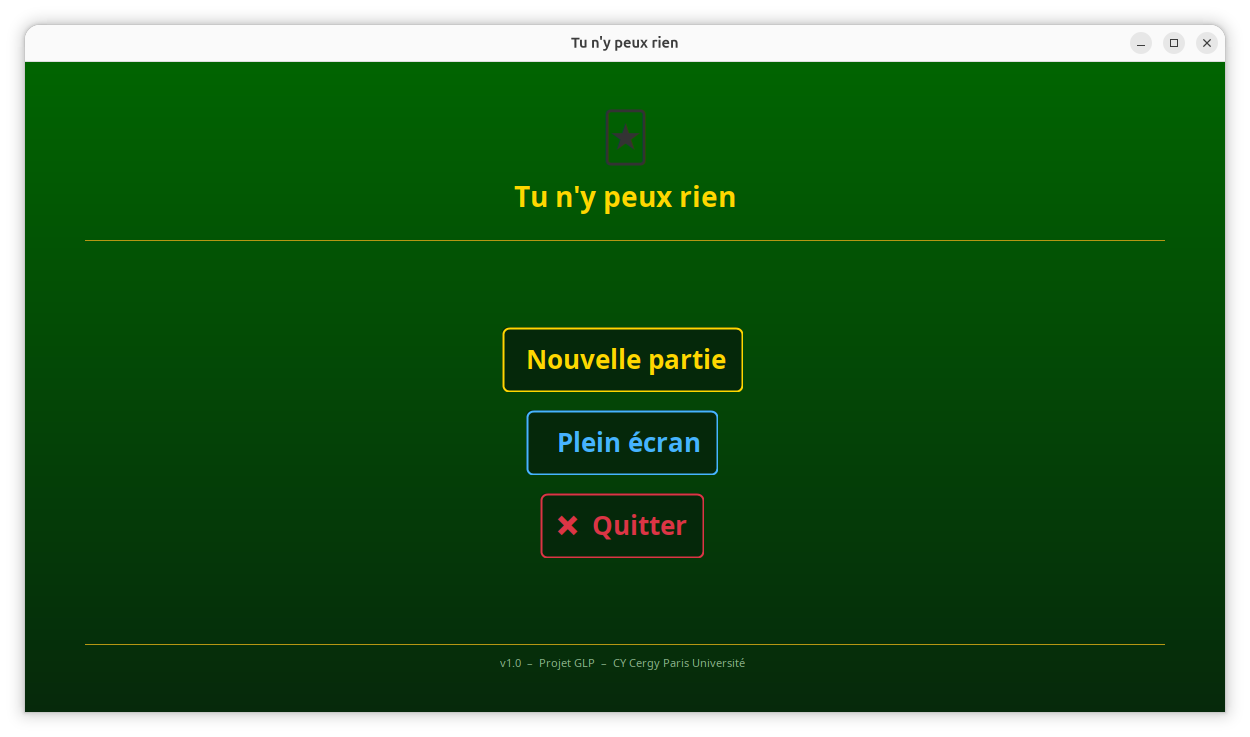
\includegraphics[width=10cm]{images/menu.png}
\caption{Menu principal}
\label{fig:menu}
\end{figure}

\subsection{Configuration de la partie}
\paragraph{} Cliquez sur "Nouvelle partie" pour accéder aux options. Sélectionnez le nombre de joueurs (3 à 5) et la difficulté des bots (Facile, Moyen, Difficile).

\begin{figure}[h!]
\centering
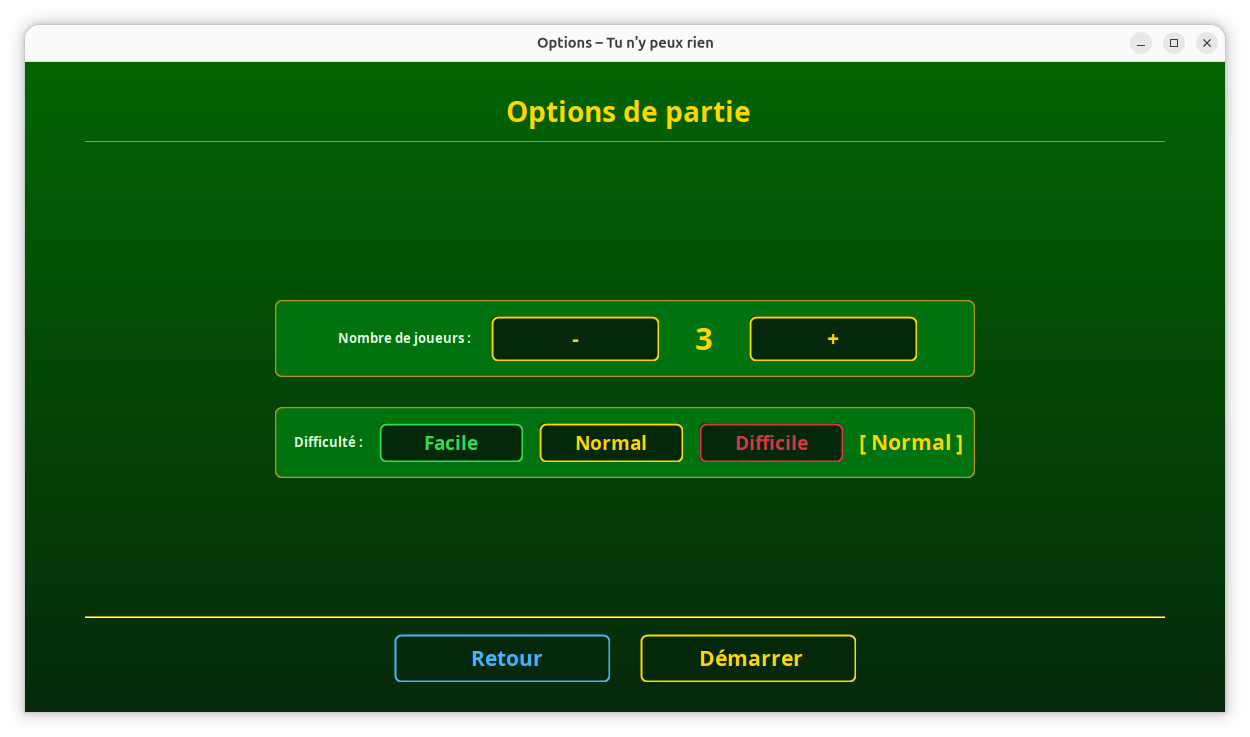
\includegraphics[width=10cm]{images/options.png}
\caption{Écran des options}
\label{fig:options}
\end{figure}

\subsection{Déroulement d'une partie}
\paragraph{} Le joueur humain est "Vous". Les bots sont représentés par des avatars. Pour jouer, sélectionnez des cartes dans votre main (clic gauche) puis cliquez sur "JOUER LES CARTES SÉLECTIONNÉES". Si vous ne pouvez pas jouer, cliquez sur "PIOCHER".

\begin{figure}[h!]
\centering
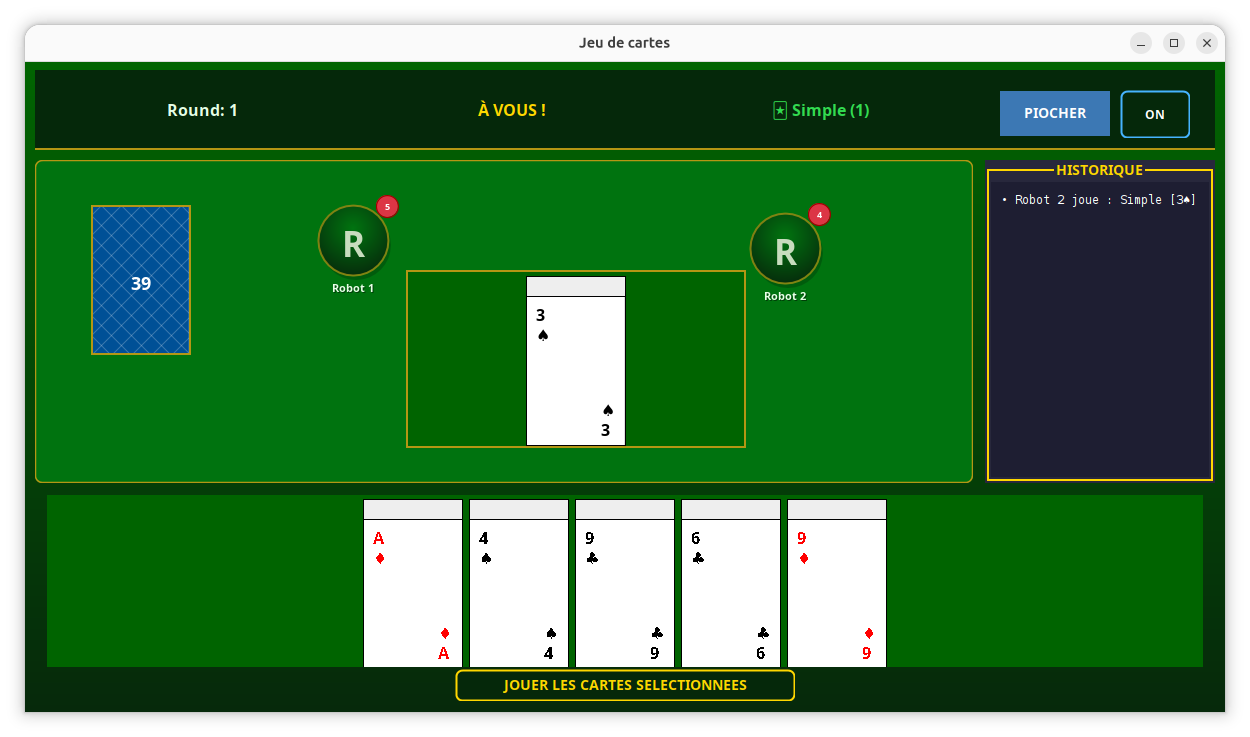
\includegraphics[width=12cm]{images/gameplay.png}
\caption{Interface de jeu}
\label{fig:gameplay}
\end{figure}

\subsection{Fin de partie}
\paragraph{} Quand un joueur n'a plus de cartes, l'écran de fin s'affiche avec le podium, les scores et les statistiques.

\begin{figure}[h!]
\centering
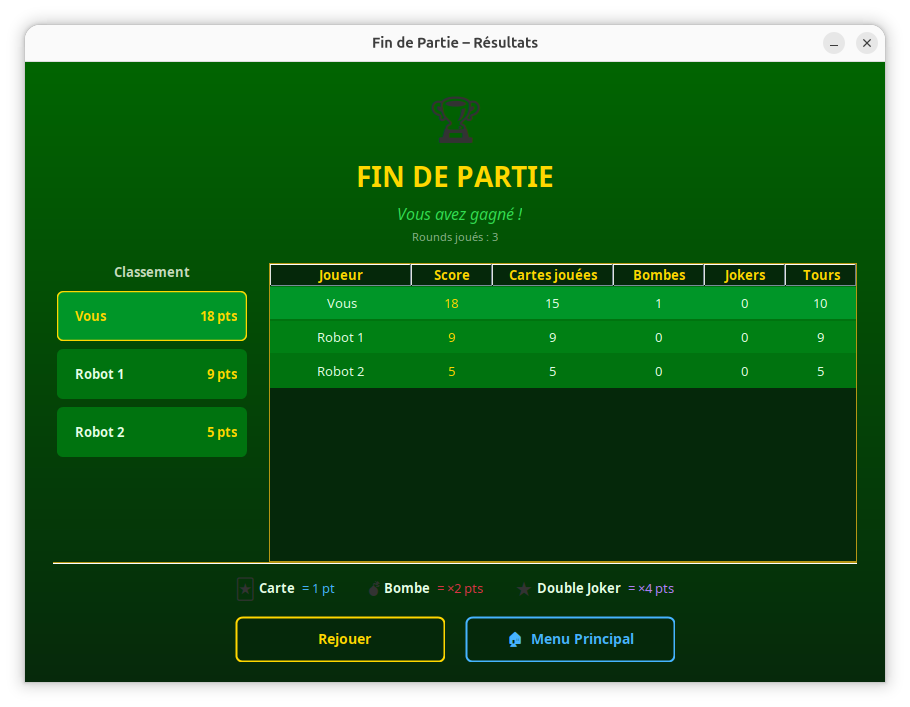
\includegraphics[width=12cm]{images/endgame.png}
\caption{Écran de fin de partie}
\label{fig:endgame}
\end{figure}
